\documentclass[12pt]{report}
\usepackage[export]{adjustbox}
\usepackage{wrapfig}
\usepackage{graphicx}
\usepackage[utf8]{inputenc}
\usepackage[margin=0.75in]{geometry}
\usepackage{hyperref} 





\begin{document}

	
	
	\begin{titlepage}    % title page begins here
		%\centering	
		%\textsc{\huge Royal University of Bhutan}\\[4cm] % Name of your university/college
%		\textsc{\LARGE \textbf{PRW301 Introduction to Research}}\\[0.5cm] % Major heading such as course name
	
		\newcommand{\HRule}{\rule{\linewidth}{0.5mm}} % Defines a new command for the horizontal lines, change thickness here
		
		\center % Center everything on the page
		
		%---------------------------------------------------------
		%	HEADING SECTIONS
		%---------------------------------------------------------
		
		


		
		%---------------------------------------------------------
		%	TITLE SECTION
		%---------------------------------------------------------
		
		\HRule \\[0.6cm]
		{ \huge \bfseries Feasibility Study On online vegetable Marketing in
Gyalpozhing}\\[0.4cm] % Title of your document
		\HRule \\[1.0cm]
		
		
		%---------------------------------------------------------
		%	GROUP & SECTION INFO
		%---------------------------------------------------------
		\begin{center} 
		\vspace{1cm}
		
		\uppercase{Research report submitted in partial fulfillment of the requirements for the module: \emph{PRW301 Introduction to Research}}\\[3cm] 
		
			{\textsc{Section: A }}  \hspace{4cm}		{\textsc{Group: 6 }} 
		\end{center}
		
		
		
		%---------------------------------------------------------
		%	AUTHOR SECTION
		%---------------------------------------------------------
		
		%\begin{minipage}{0.4\textwidth}
		\begin{center} \large
			% \emph{Authors:}  
			\medskip
			{\textsc{Dawa Tshring }}  \quad  {\textsc{Dhendup Ghishing}} 	\quad
			{\textsc{Kezang Dorji }}  \quad  {\textsc{Nar Bdr }}   % Your name in small caps
		\end{center}
		%\end{minipage}
		
		\vspace{2cm}
		
		%---------------------------------------------------------
		%	DATE SECTION
		%---------------------------------------------------------
		\begin{center}
			{\large 22/12/2020}		% Date, change the \today to a set date if you want to be precise
		\end{center}

		
		%---------------------------------------------------------
		%	LOGO SECTION
		%---------------------------------------------------------
		%\vfill

		%---------------------------------------------------------
		%	LOGO SECTION
		%---------------------------------------------------------
	
	 
		\begin{figure}
		\centering
		
\includegraphics[width=0.14\textwidth]{RUB_logo}  % Include a department/university logo -  the graphicx package needed	
		\hspace{5cm}	
		
\includegraphics[width=0.21\textwidth]{gcit_logo.png}  % Include a department/university logo -  the graphicx package needed	
		\vspace{1cm}	
		\end{figure}
	
		
		\vfill % Fill the rest of the page with whitespace
		
		
		
		\large
		\textbf{Module tutors}:  \hspace{1cm} Mulualem Teku \hspace{1cm} Tashi Phuntsho
		
	%	{\rule{11cm}{0.2mm}}
		
	\end{titlepage}               % title page ends here 
	
	

%----------------------------------------------------------
% The ABSTRACT section 
%----------------------------------------------------------

\begin{abstract}
In the past years the intensification of competition has change the way how marketing communicates with customers, sellers and farmers.In this regard, our team has concern regarding the efficiency of vegetable marketing in Gyalpozhing. It is believed that poor efficiency in marketing strategy is fluctuating customer's prices, spreading illness and small proportion of customer's money reaching to farmers and sellers. Similarly there is no other means to buy and sell vegetable other than traditional vegetable marketing(Current Vegetable Marketing) in Gyalpozhing. Due to such challenges in Gyalpozhing, the team has done research on feasibility of online vegetable marketing.\newline\\[0.1cm]
In this research, the team has focused on three major factor i.e, knowledge about online application, internet accessibility, and trust towards online vegetable marketing  to determine the feasibility of online vegetable market. We have taken these three factors because it is must that one should know about online application as new marketing strategy which will be based on online application. Internet accessibility also plays key role in online vegetable marketing because without internet one cannot operate online application. Finally to do online marketing one should have trust on online marketing. Without having trust over online marketing we cannot proceed with online marketing, so it becomes necessary for all sellers, farmers and customers to have trust over online marketing system to implement it.\newline\\[0.1cm]
The research is based on predictive analysis  which favors in answering the questions of future  prediction using previous and current data. All required data are collected from farmers, sellers, and customers of Gyalpozhing through interviews to retrieve precise data. This analysis is taken into two phases i.e, qualitative and quantitative analysis. In qualitative analysis we have included direct statement given based on interview questions from all the sellers, farmers, and customer.In other hand, in qualitative analysis we have taken certain numbers of sellers, farmers, and customers who have trust towards online application, how many of them know about online application and how many of them have internet connectivity.Through these data, we have figure out the feasibility of online vegetable marketing in Gyalpozhing.

\end{abstract}



\pagenumbering{roman}

\tableofcontents			% add table of contents 

\newpage
	

\pagenumbering{arabic}




\begin{normalsize}		
		
		
%---------------------------------------------------------
%	chapter: Research Overview 
%---------------------------------------------------------		


\chapter{Research Overview}
\label{chapter_overview}
\section{Introduction}
The global economy and the organization from different parts of the world have witnessed tremen-
dous changes in the last three decades with technological advancement in online marketing. Online
vegetable marketing has driven the ideas of traditional marketing to the advanced system. The
new application and ideas are already available to the general public but there is much space to
learn and keep on upgrading. The idea of online marketing is instantly flourishing over the world
fulfilling the basic needs of the people. The system of online marketing was launched within Bhutan
from the past few years and it is overwhelming contributing in the living standard of the people
in Bhutan. Over the time, the demand for the online application system is growing in the country
where all citizens are into the advanced system with the new features. On the other hand such
applications system are able to solve the problem of unemployed youths in the country.\newline\\[0.1cm]
In online marketing, people can advertise and reserve the product over the internet and get the
required product at the quick instant of time. This application system is fast and efficient as it
provides detailed information on the vegetables, services and offers of the seller. Moreover in such
type of marketing the time of the seller, as well as the time of the customer is saved as both the seller
and customer do not have to meet face to face in the market. This business provides a platform for
the customer to reserve the vegetables and the seller to advertise the vegetable from any place at
particular instant of time within the range of the market.\newline\\[0.1cm]
On believing the concept and fact of online vegetable marketing, the team builds the curiosity to
learn and see the feasibility of online vegetable marketing in Gyalpozhing. In Gyalpozhing, every
weekend people have to gather in the vegetable market and to do the necessary shopping of veg-
etables for the rest of the days. In this situation, it becomes hard for people of Gyalpozhing to get
vegetables of the right diet as many people rush to get vegetables at once. The time limit for buyers
and sellers to do market is very less as there are many customers in Gyalpozhing. More importantly
due to huge gathering every weekend there is also a high risk of spreading diseases. However, to
sell their vegetable in market, farmers have to store their products in stock which spoils the quality
and freshness of vegetables, as a result, it deteriorates the price of vegetables.\newline\\[0.1cm]
Due to such problems as mentioned above, our team is going to find whether there is a need for
online vegetable marketing in Gyalpozhing. Online vegetable marketing would ease marketing strategy and would solve the problems of spreading diseases in a community and time consumption for
marketing would be reduced for both sellers and buyers. So based on these statements the team
would be researching the feasibility of an online vegetable market in Gyalpozhing.



%---------------------------------------------------------
%	Objectives
%---------------------------------------------------------		

\section{Objective}

The main objective of this study is to figure out the feasibility of online vegetable marketing in
Gyalpozhing. In addition, to dig out the different behavior and the reaction of the customer and
seller dealing online application. Similarly, research will help the reader to understand how online
vegetable marketing will reduce the risk of spreading diseases and time consumption for marketing. \newline\\[0.1cm]
The conducted studies of the World Health Organization show that the adoption of a healthy
lifestyle includes a diet rich in vegetables which promotes the strategy to reduce chronic diseases.
Knowing fact that rich diet vegetable has a great impact on our daily life, do we bother to take it
for a healthy life. Similarly, it becomes impossible for many people to produce enough vegetables
due to their different professions. It has become necessary for those people to get vegetables from
the market. In traditional vegetable marketing, we have witnessed that consumers and sellers
rushing to the vegetable market every weekend specifically in Gyalpozhing. Every weekend there is
a huge gathering in the vegetable market in the scene, we again notice it is an unhealthy practice
of marketing.Due to huge gatherings, there is always a risk of spreading diseases.\newline\\[0.1cm] 
Similarly, there is always a chance that vegetables may get ruined if the vegetables are only sold on weekends. The vegetable
may get ripe or ready on other days, by the time seller wants to sell their product it may get
ruined or rotten. On the other hand, consumers are not getting the right product at the right time
although the seller sells the product and the consumer buys the product, there is always a risk
that the consumer is living an unhealthy life. Those problems are tackled by online marketing system in
other parts of the nation and  satisfying the needs of customers. In Gyalpozhing,
such an application is not launched yet.There fore our team would like to check feasibility on online vegetable marketing in Gyalpozhing. \newline\\[0.1cm]

{\bfseries Research question}\newline\\[0.1cm]
1. How online vegetable market satisfy the wants and need of the customer and seller?\newline\\[0.1cm] 
2. What are the main reason for studying the feasibility of online vegetable marketing?\newline\\[0.1cm] 
3. Will online vegetable marketing become user friendly in Gyalpozhing?\newline\\[0.1cm] 
4. Do customer have interest in online marketing?\newline\\[0.1cm] 



%---------------------------------------------------------
%	Scope and Limitation
%---------------------------------------------------------		

\section{Scope and Limitation}
{\bfseries Scope }\newline\\
Our scope is limited to Gyalpozhing, Mongar since it is center advancing for farmers, customers, and sellers for marketing vegetable. Moreover, population count is also high in Gyalpozhing town compared to other part. Which is why demand from customers will be also high on vegetables, and number of sellers will also increase. \newline\\[0.1cm]
{\bfseries Limitation }\newline\\
Although, online marketing allows a wider reach, some challenges were faced while doing this research. In particular, the team had hard time while conducting interviews with farmers, sellers and customers. Sometimes the team was not able convince the questions to them and unexpected respond was collected, which resulted tougher data cleaning . Though many of them were supportive and responsive to the research team but some of them were reluctant to answer the interview questions.


%---------------------------------------------------------
%	Significance
%---------------------------------------------------------		

\section{Significance}

Feasibility studies on online vegetable marketing allows to address where and how it will operate. It determines the viability of online vegetable market ensures technical feasibility which is accepted by community. It also ensures that feasibility of online vegetable marketing in Gyalpozhing before implementing it. This research will benefit those investors who want to implement online vegetable marketing in Gyalpozhing. Moreover there is no alternate way for customers and seller to buy and sell vegetable.  Alternatively, if online vegetable marketing is launched, all sellers, farmers and customers would be benefited and vegetable marketing would be eased.\newline\\[0.1cm]
Challenges like huge gathering, spreading of diseases and limited space in vegetable market would be solved if online vegetable is launched. Thus to achieve these benefits, it becomes first and foremost thing to check the feasibility of online vegetable marketing.








%---------------------------------------------------------
%	chapter: Literature Review
%---------------------------------------------------------		

		
\chapter{Literature Review}			

The Internet has proved its capabilities for many individuals and organizations for the marketing
of their products. The objective of the internet in any business is to expand the business to
maximum customers and to minimize the effort in the distribution channel. Developing the use of
the internet in business is no easy task for organizations as they are required to established new
and different marketing strategies. Information technology tools have been verified and accepted
commonly to answer the problem of marketing faced by farmers. In the present era of globalization,
trade liberalization and privatization, information technology like email, e-banking, internet, and
e- commerce. The Internet is the fastest developing communication medium on earth at present.\newline\\[0.1cm]
Around the world, consumers are increasingly becoming aware of vegetables and their perceived
benefits. The trend is growing fast especially in the developed world facing the USA \cite{key1} (Greene, 2000),
Europe(food and agriculture organization, 200). \cite{key2}Gil, Gracia Sanchez (2000) have investigated that
consumers are getting health conscious and are paying more attention to the quality of vegetables
consumed. During the last decades concern toward health, safety, and nutrition has increased ever
so sharply.\newline\\[0.1cm]
The current farmer's marketing strategy would impact the customers and sellers thus the marketing strategy should shift towards online marketing where farmers don't have to be fully seller\cite{key3}(Carmer, 2012).
Unlike in the past, most farmers need not have to travel to the border towns to sell their vegetables.
Since June 18, Bhutan food cooperation limited has started buying a vegetable product from farmers
to reduce time and their energy. A team of young graduates with agriculture and civil engineering
background began selling vegetables online through their website called Bhutan Smart Shop \cite{key4}(BSS).
The news collected or reporter Sonam says that their team response was positive and
encouraging since they can sell their vegetable successfully online within Bhutan.\newline\\[0.1cm]
Kencho Tobgay the founder of online vegetable marketing in Bhutan (BSS) said that “he has come
across huge traffic congestion at a centenary farmers market, especially weekends. It was also
difficult to get parking space.” They feel that their services will be the solution to this problem
faced by the residents of Thimphu(Capital) and contributes to reducing pollution.\newline\\[0.1cm]
The team said that the online shopping sites would also assist users to manage and see the record
of their expenses. This will help their expenses and make them financially conscious. So, BSS plans
to grow vegetables in near future. Finally, conclude by saying these services of online marketing
will be spreading through all the dzongkhag.



\newpage
	
\chapter{Data Analysis and Discussion}	
\label{chapter_analysis}		
		
%---------------------------------------------------------
%	Methodology
%---------------------------------------------------------		

\section{Research Methodology}
This research study is divide into two-part, the pilot study, and the main study. A pilot study is base on the exploratory research which will be conducted based on interviews in order to get the required data. We have conducted a baseline interview in Gyalpozhing and ask the people residing within the Gyalpozhing to give their opinion on online vegetable marketing, as per the pilot phase we have evaluated their requirements and satisfaction.\newline\\[0.1cm] 
The main study is based on quantitative method and qualitative method, where we have conducted interview with various
people of Gyalpozhing and noted their direct statement and opinion through live interaction. In quantitative method we have collected the data such as number of framers, sellers and consumers who are interested and willing to market through online. And to collect data simple random sampling method was used as the team has randomly picked sellers, farmers and customers to interview. The analysis was done based on predictive analysis which favors in answering the questions of future outcome. As our aim is to check the feasibility of online vegetable market using the current and previous data to make the future prediction.  





%---------------------------------------------------------
%	Methodology
%---------------------------------------------------------		

\section{Results and Discussions}

{\bfseries Quantitative Analysis }\newline\\[0.1cm]
To check the feasibility of online vegetable marketing in Gyalpozhing, Mongar, the team has done an analysis based on a methodology that was stated in the proposal of the research. Firstly the team has thoroughly discussed the questions which needs to be asked while conducting interviews with farmers, sellers, and customer. After successfully setting up the interview questions inline with the objectives of the research, the  team has done interviews based on  simple random sampling technique in Gyalpozhing. All the required information and data were recorded in the paper. Additionally the team has also captured some of the videos of interviews as evidence and the link of video is placed in appendices section.\newline\\[0.1cm]
\begin{figure}[!htb]
   \begin{minipage}{0.48\textwidth}
     \centering
     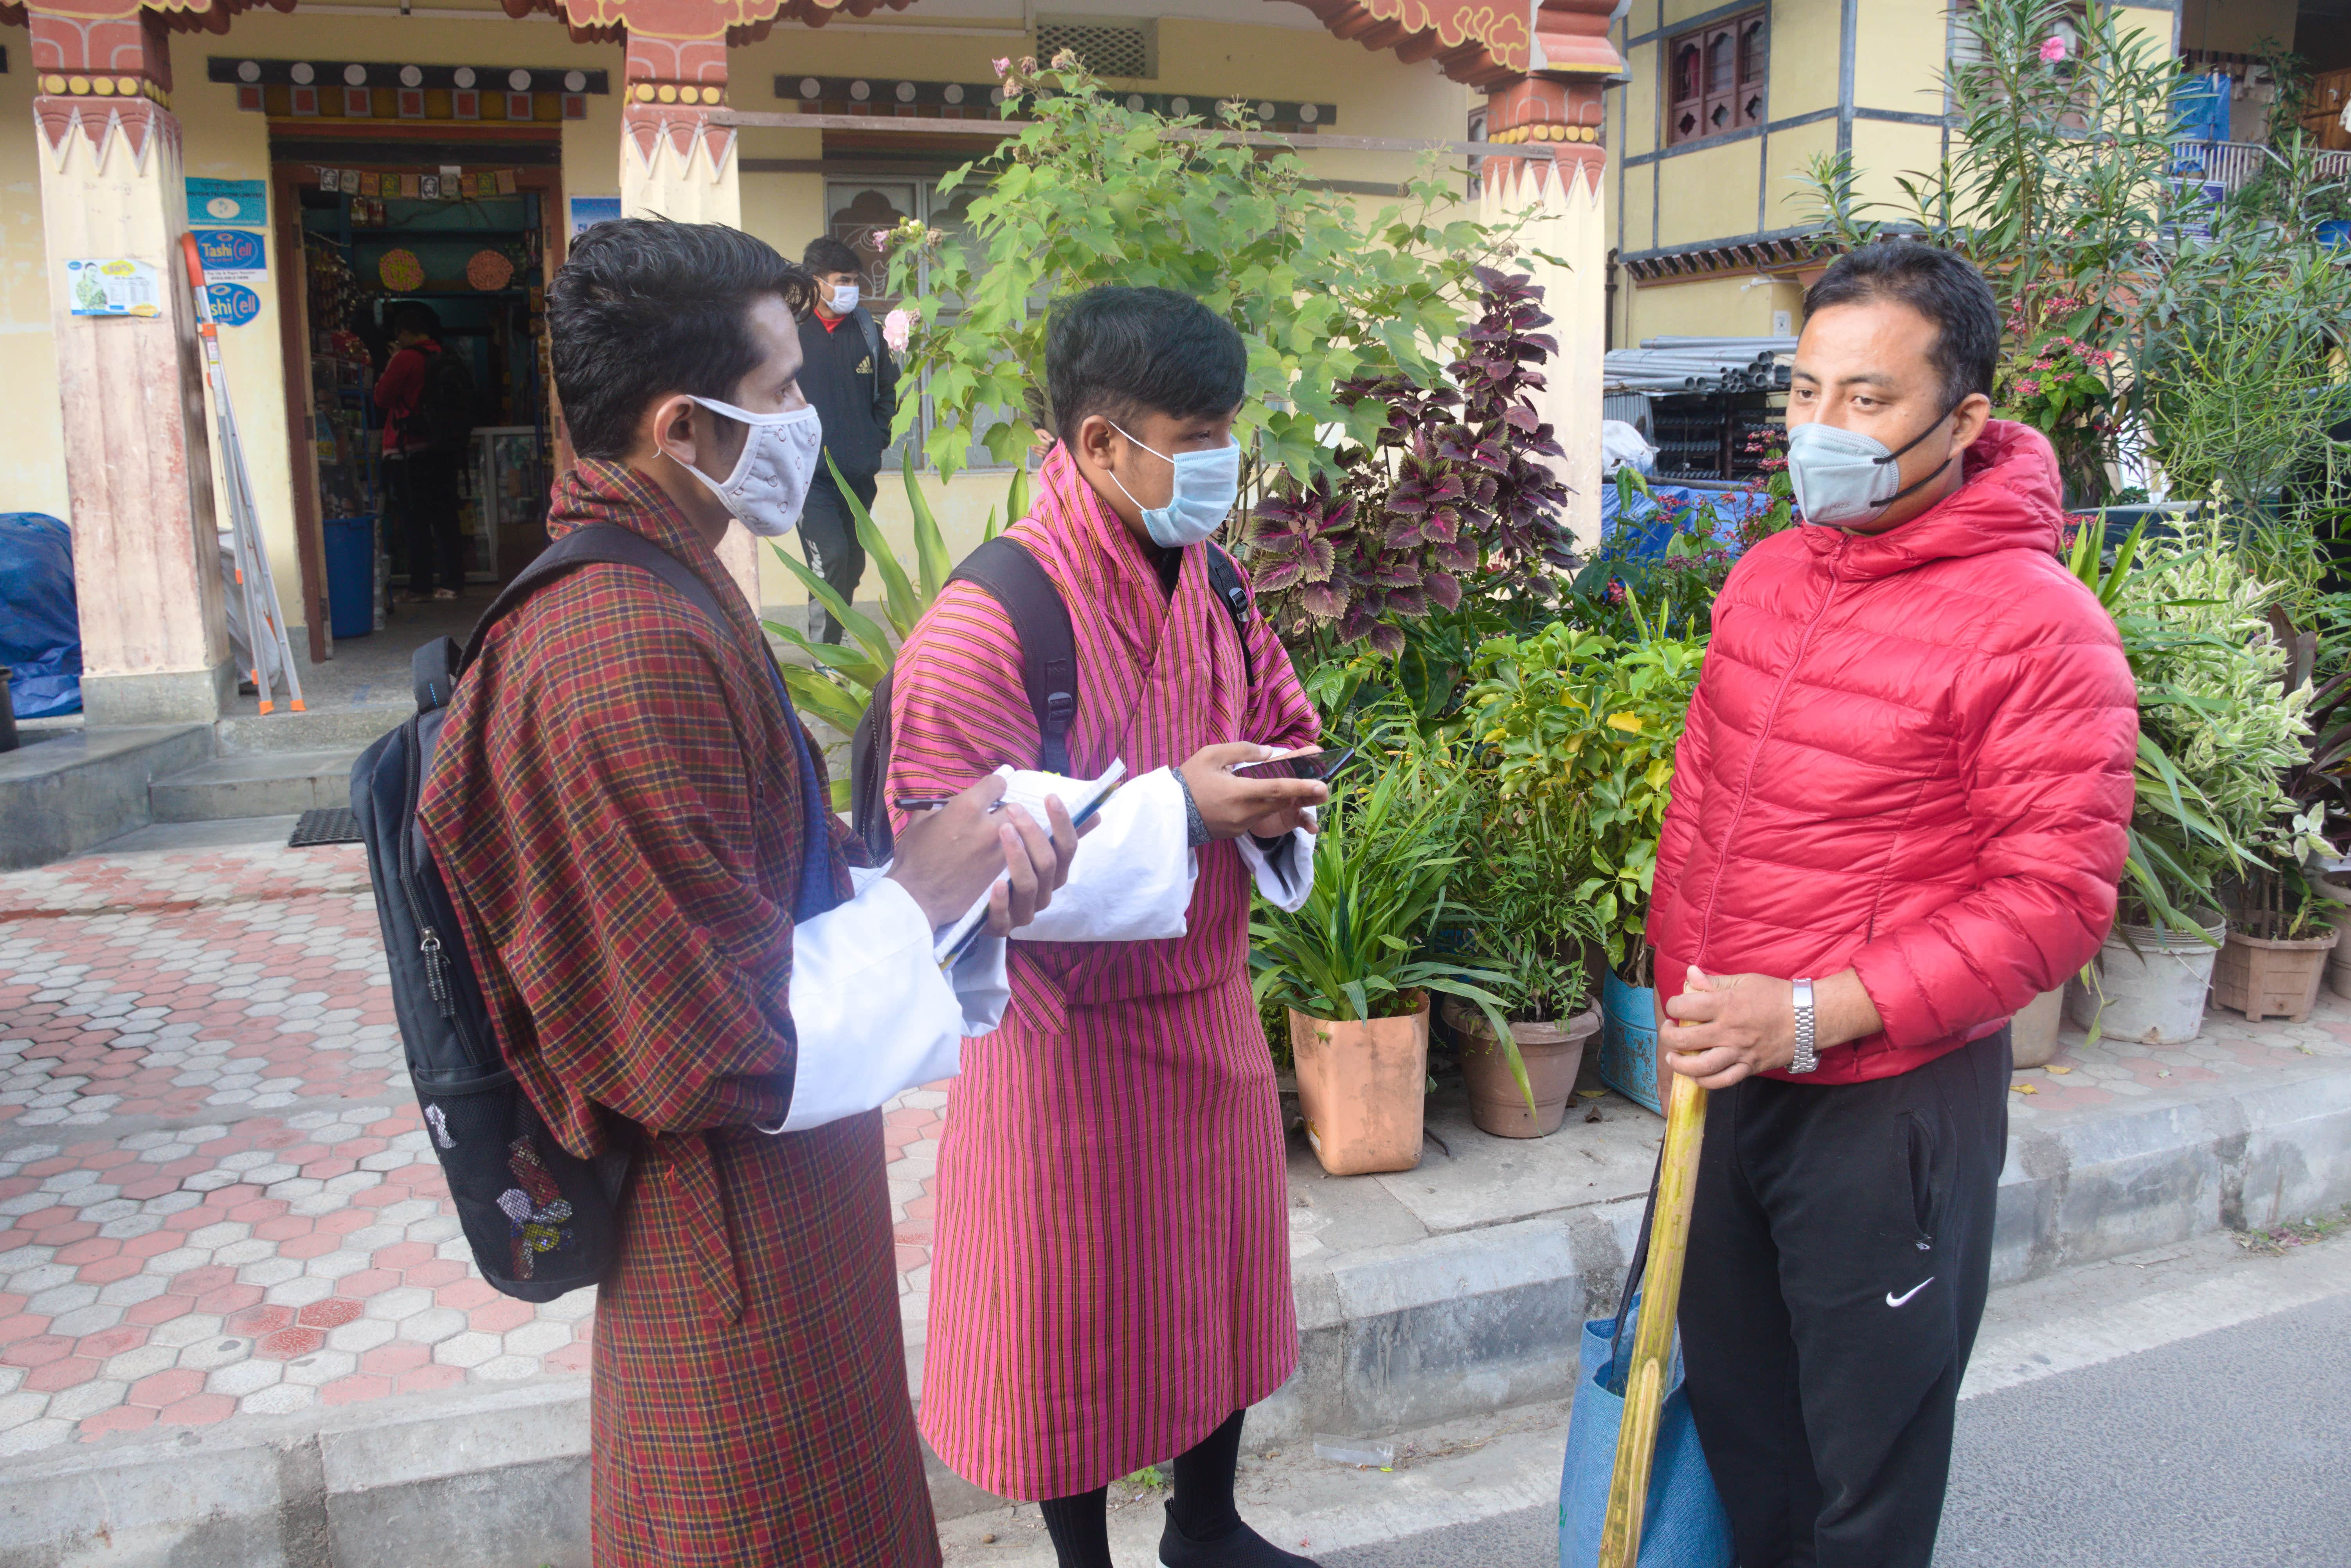
\includegraphics[width=.7\linewidth]{1-min.jpg}
     \caption{Nar Bdr and Kezang Dorji \newline interviewing with customer}\label{Fig:Data1}
   \end{minipage}\hfill
   \begin{minipage}{0.48\textwidth}
     \centering
     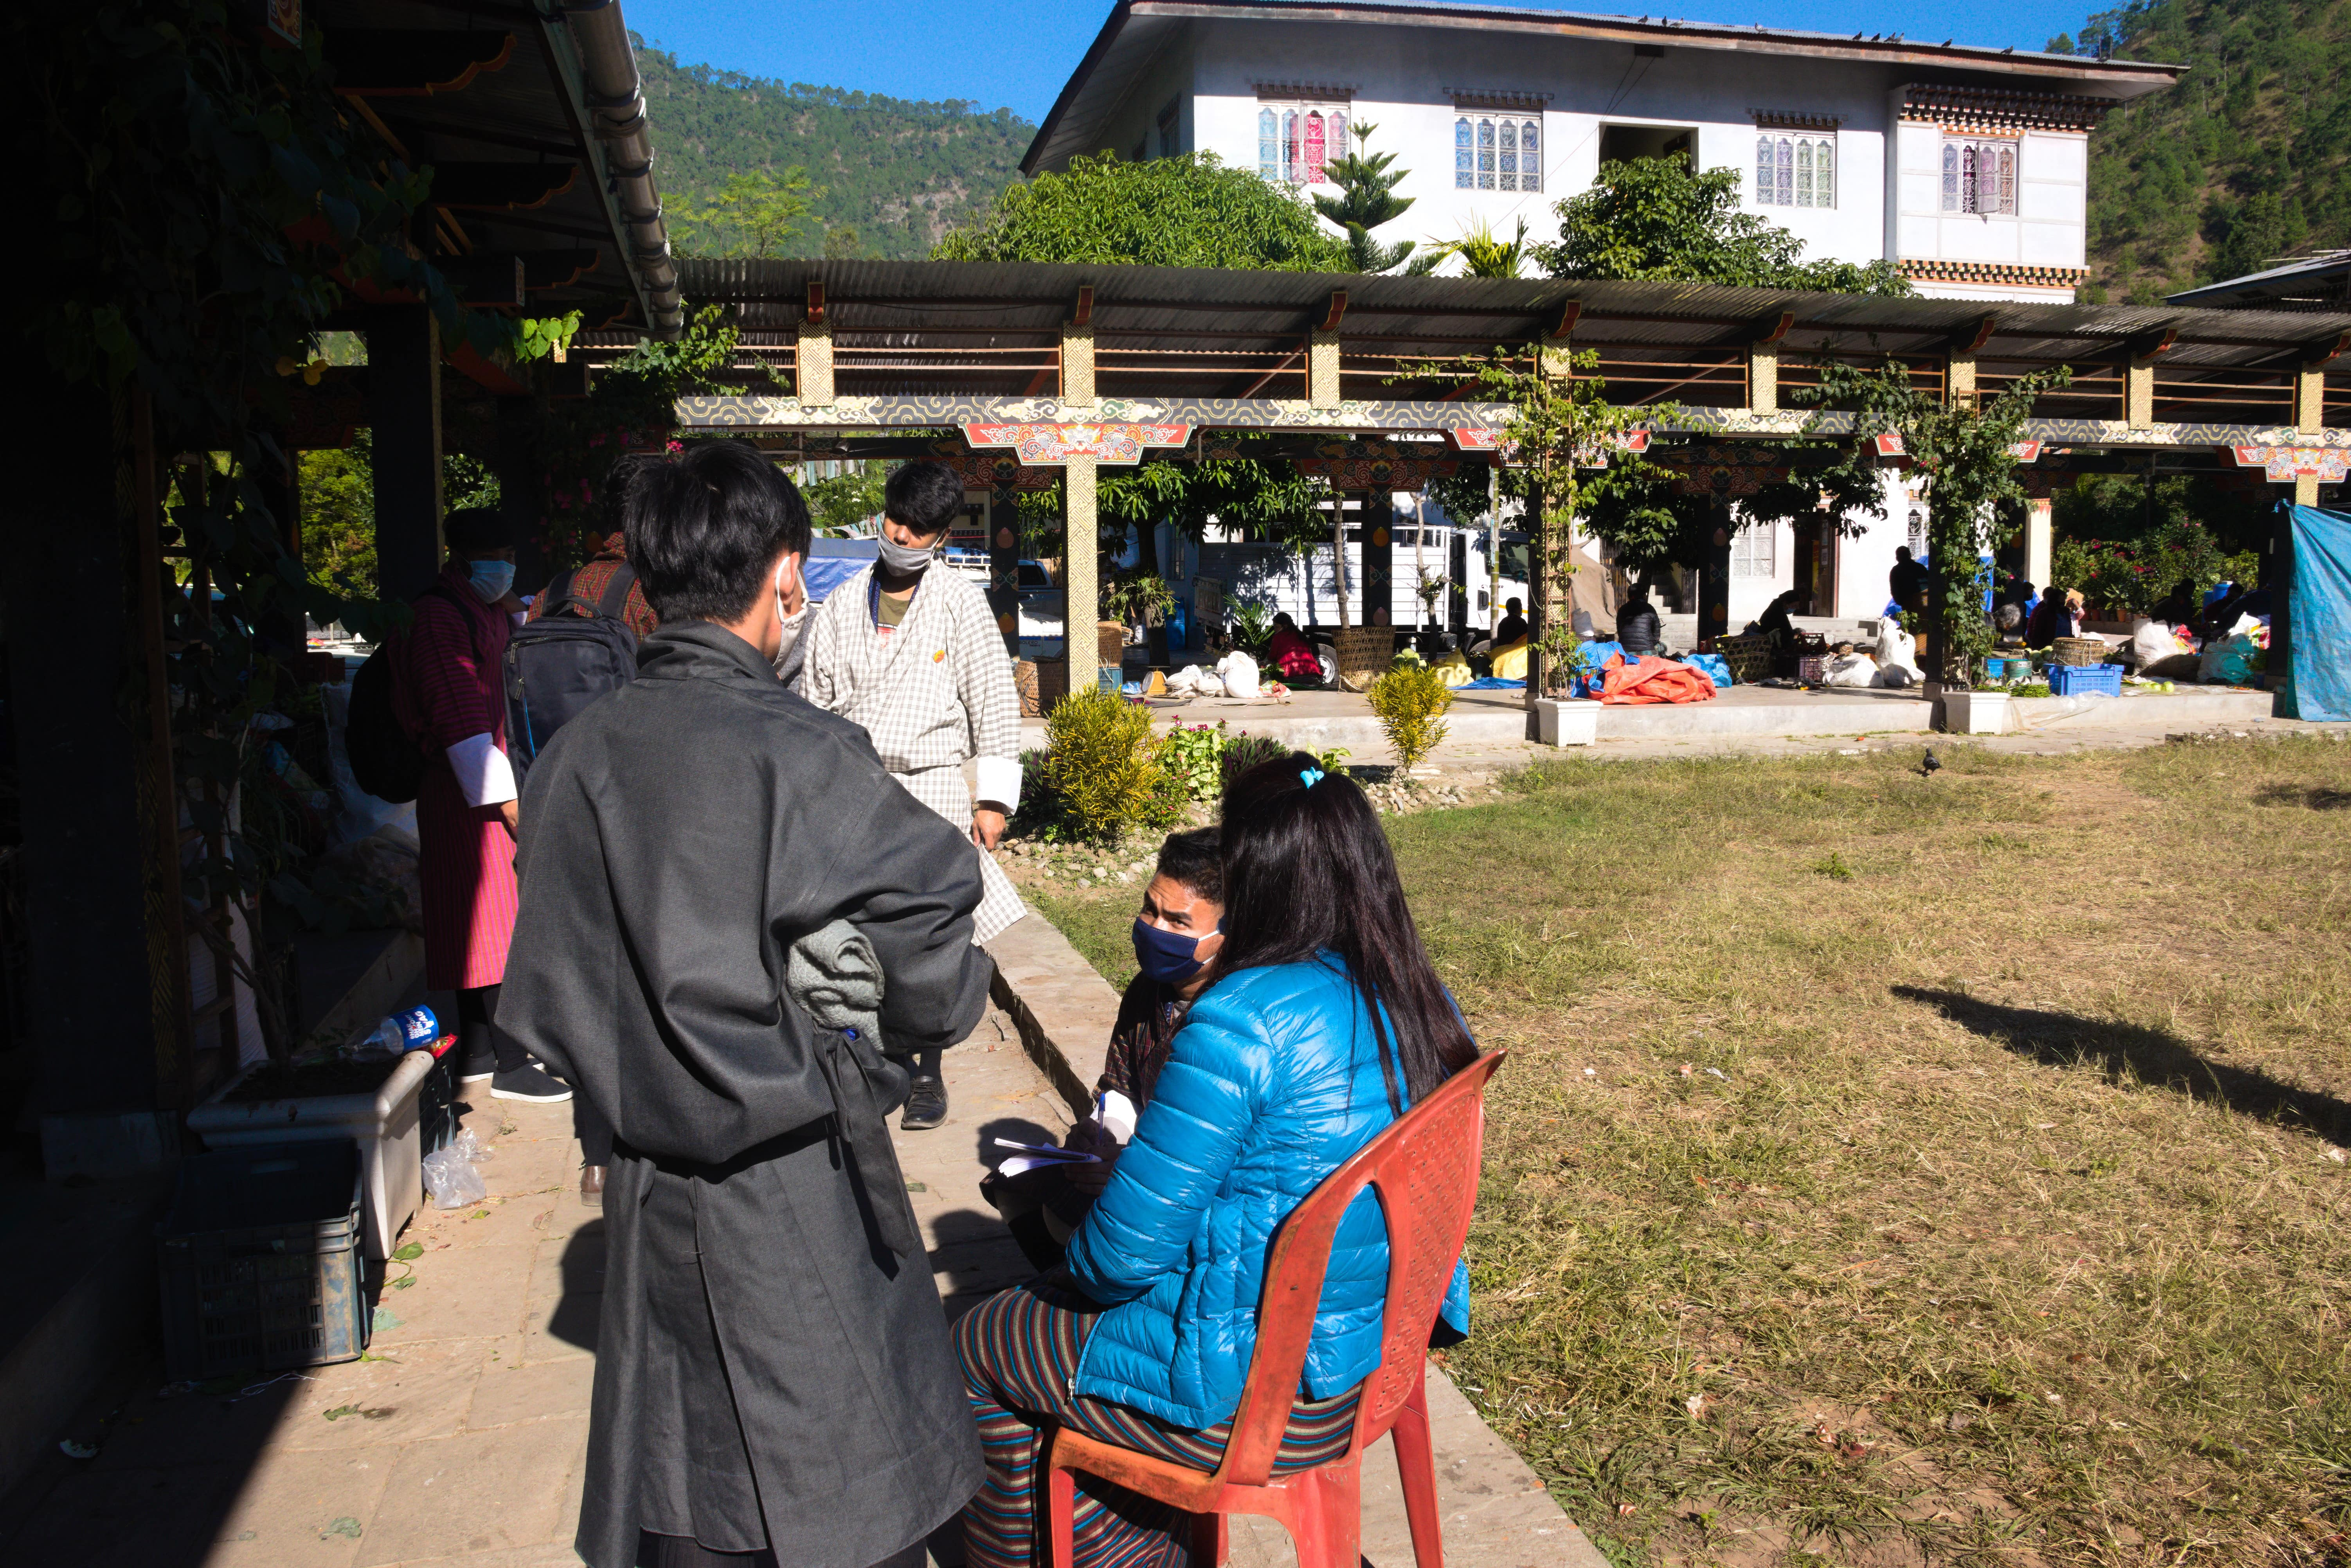
\includegraphics[width=.7\linewidth]{2-min.jpg}
     \caption{Dawa Tshring and Dhendup Ghishinginterviewing with seller}\label{Fig:Data2}
   \end{minipage}
   \begin{minipage}{0.48\textwidth}
     \centering
     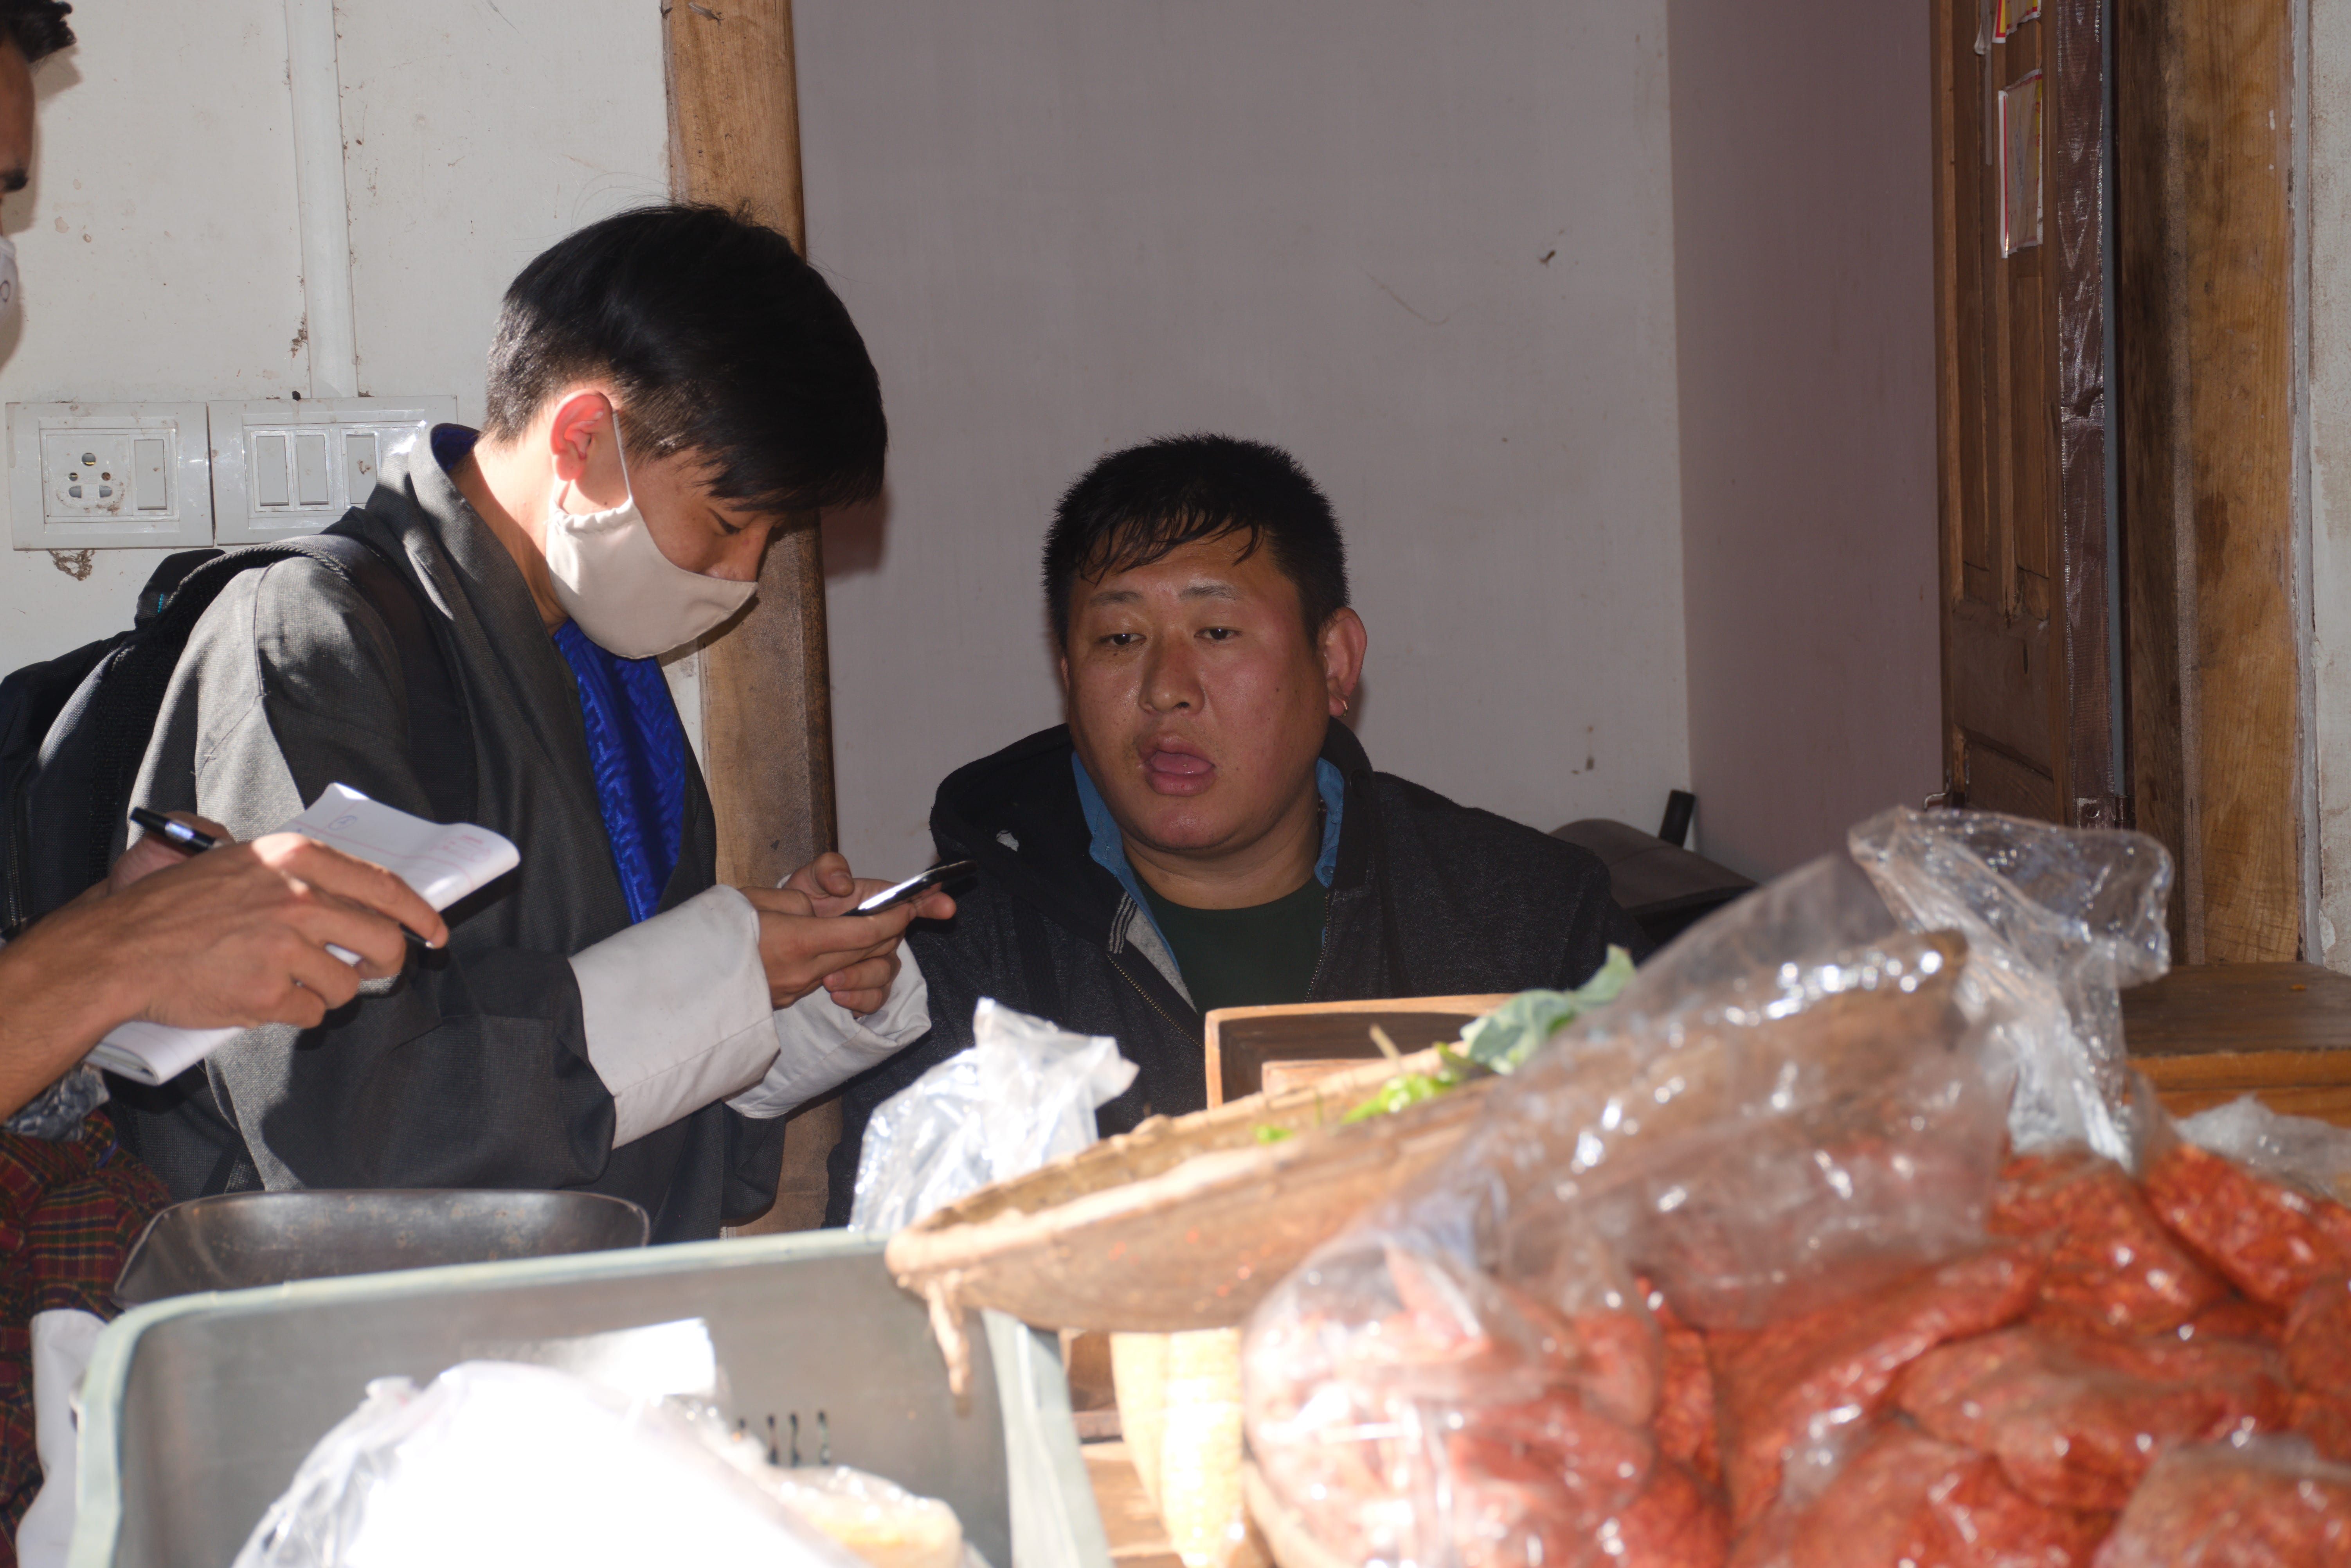
\includegraphics[width=.7\linewidth]{3-min.jpg}
     \caption{Dawa Tshring interviewing\newline with Seller}\label{Fig:Data2}
   \end{minipage}
   \begin{minipage}{0.48\textwidth}
     \centering
     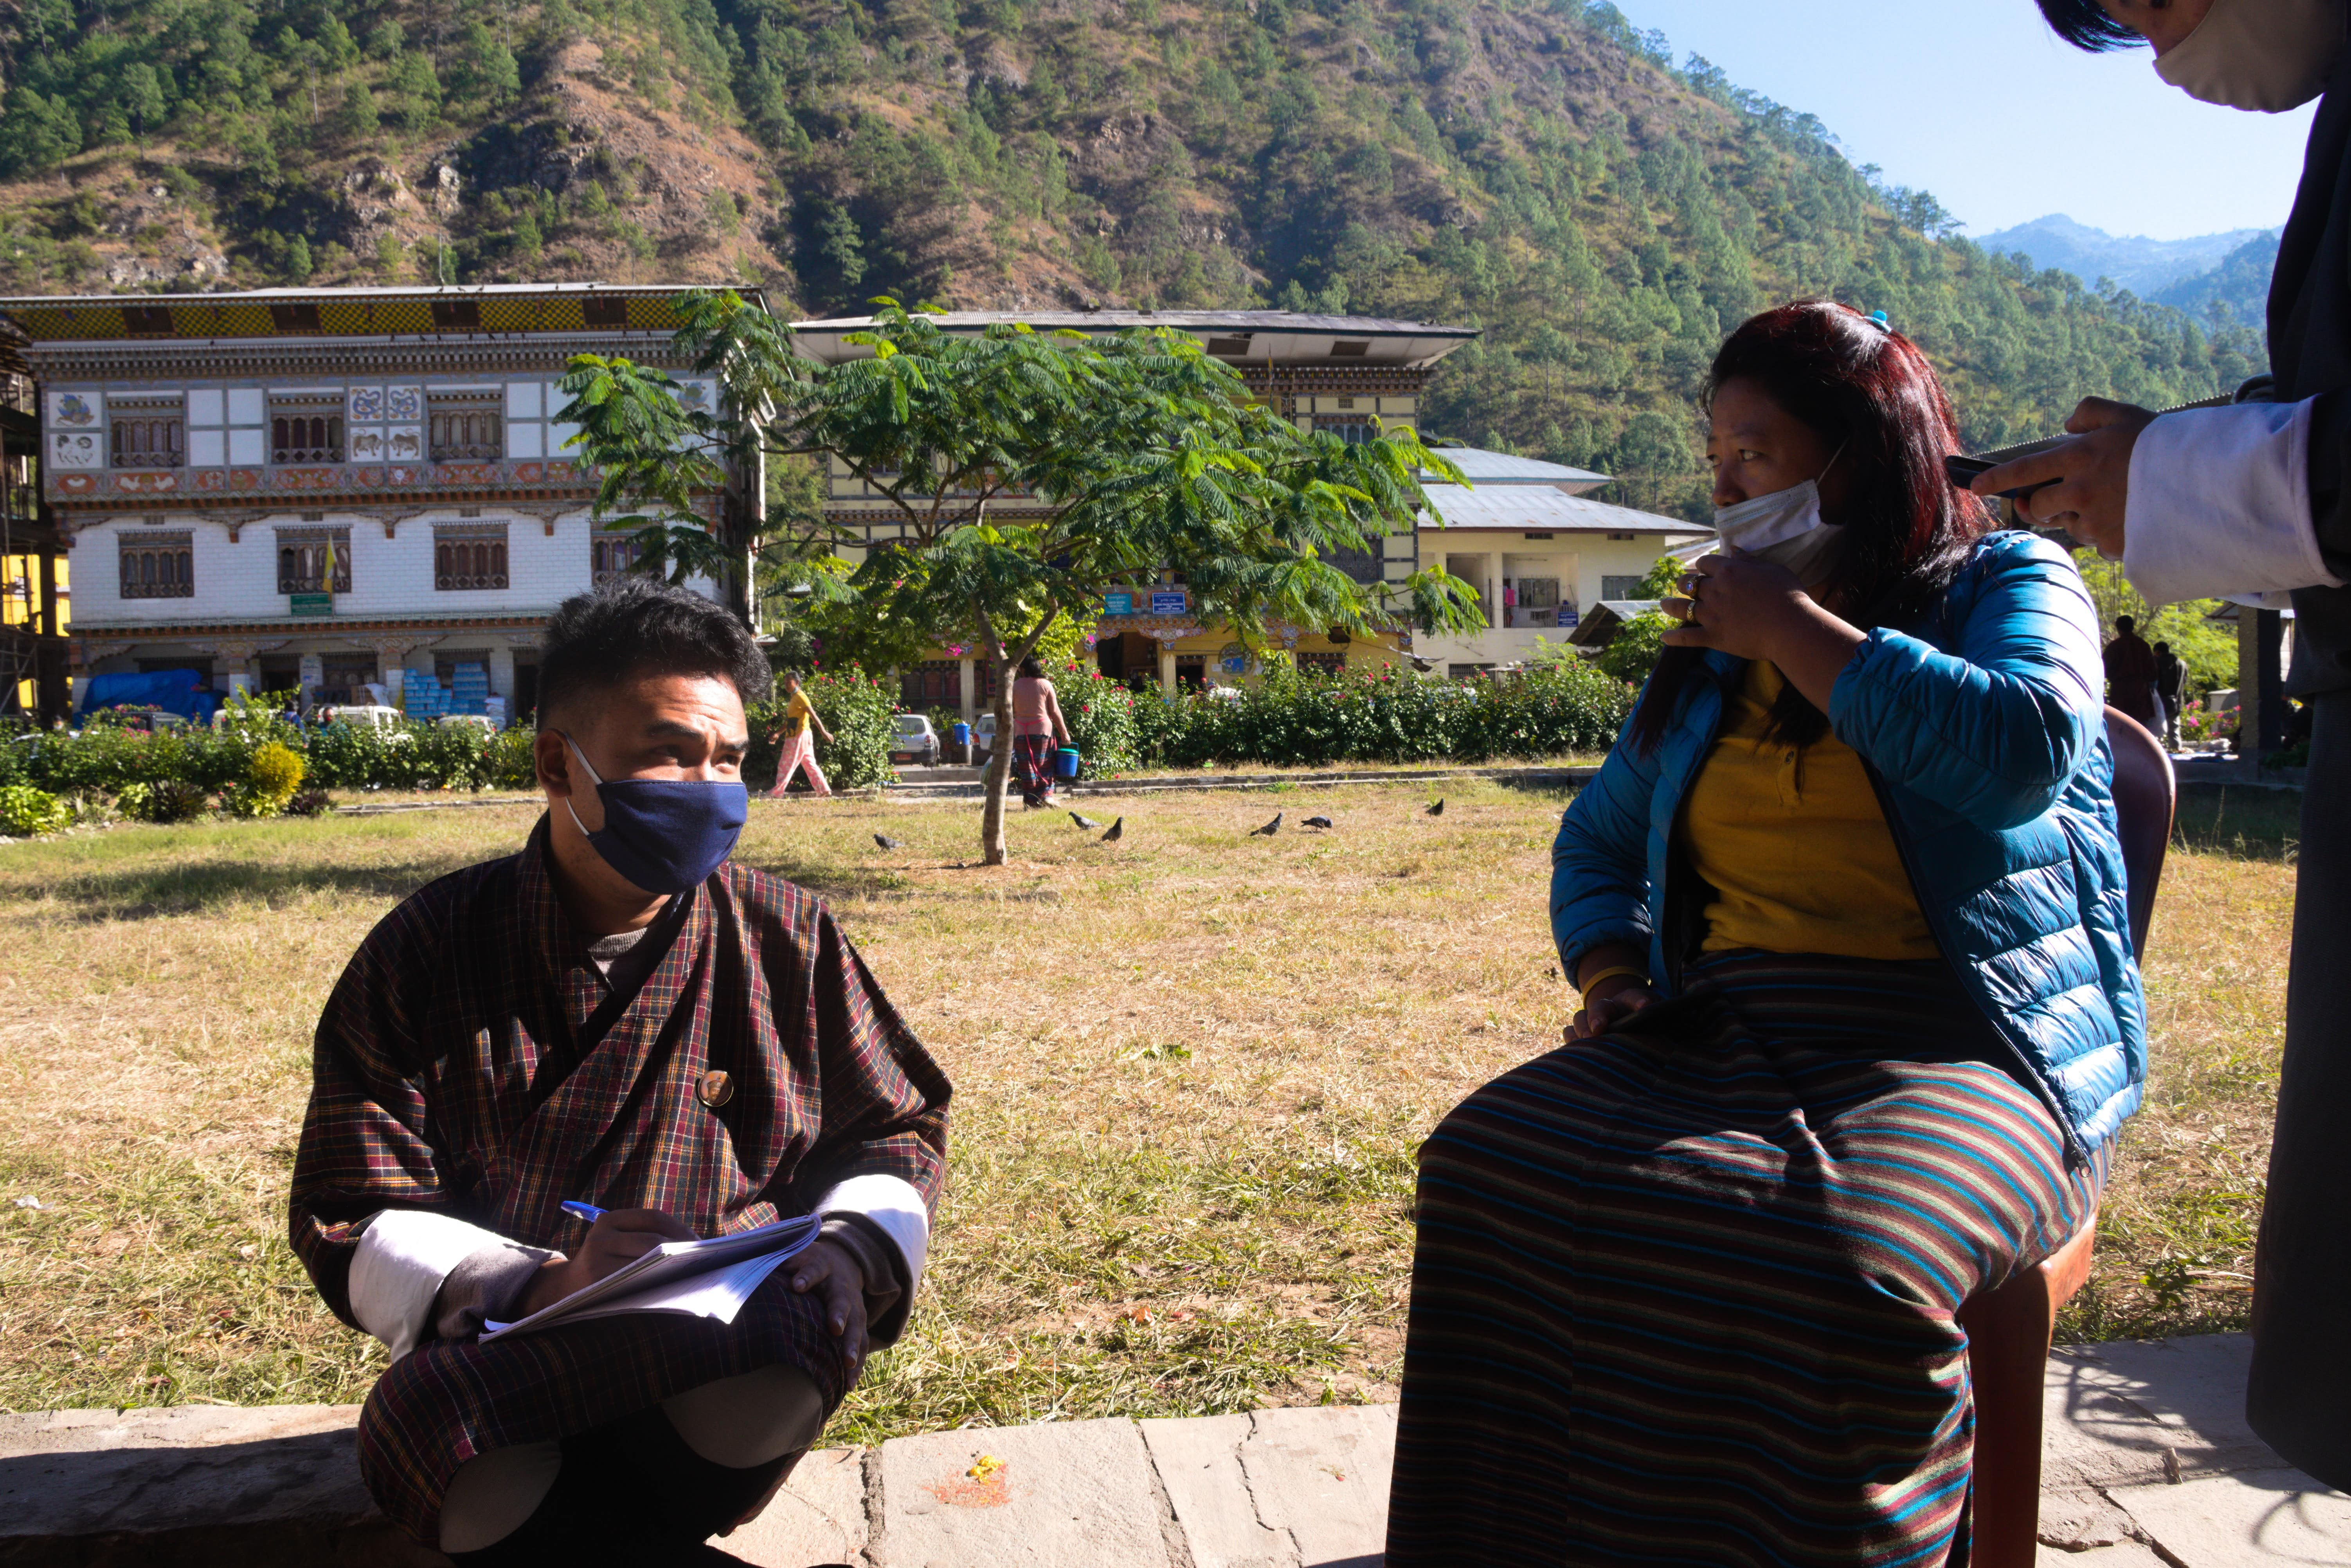
\includegraphics[width=.7\linewidth]{4-min.jpg}
     \caption{Dhendup Ghisihing interviewing\newline with farmer}\label{Fig:Data2}
   \end{minipage}
\end{figure}
In the interview, questions were asked in three phases namely to farmers, customers, and sellers. Of several questions, following questions were considered to be a major factor on account to check the feasibility of online vegetable marketing in Gyapozhing: \newline\\[0.1cm]

1)Are you able to access internet from your place?

2)Do you have any knowledge about the online application ?

3)Will you be able to trust if there is online vegetable marketing system?\newline\\[0.1cm]

\newpage
As per the respond recorded from the interview following data were figured out:\newline\\[0.1cm]
{\bfseries Seller }\newline\\
1. Do you have any knowledge about the online application ? \newline\\[0.1cm]
\begin{table}[h]       % insert the table here (where it is declared)
		\centering
		\begin{tabular}{ | l | c | r | } \hline
		\textbf{Number of Yes} & \textbf{Number of No} & \textbf{Total Number} \\ \hline			
		10 & 1 & 11 \\ \hline
		\end{tabular}
		\caption{Displaying the number of sellers who responded yes and no respectively to above question}
		\label{1.0}
	    \end{table}
\begin{figure}[h]       % options: t for top of page, b for bottom, h for current position
	\centering
	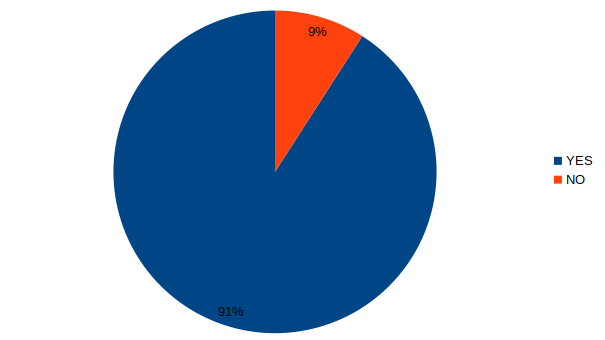
\includegraphics[width=0.5\textwidth]{seller 1.png} 
	\caption{Graphical representation of sellers who have knowledge about online application }
	\label{myLabel}		% used to reference this figure from anywhere in the document using the \ref command. 
	\end{figure}
\newline\\[0.1cm]Out of 11 sellers, 10 of them know online application resulting 91\% and 1 of them does not have knowledge of online application resulting 9\% respectively.\newline\\[0.1cm]
2)Are you able to access internet from your place? \newline\\[0.1cm]
\begin{table}[h]       % insert the table here (where it is declared)
		\centering
		\begin{tabular}{ | l | c | r | } \hline
		\textbf{Number of Yes} & \textbf{Number of No} & \textbf{Total Number} \\ \hline			
		11 & 0 & 11 \\ \hline
		\end{tabular}
		\caption{Displaying the number of sellers who responded yes and no respectively to above question}
		\label{2.0}
	\end{table}
\begin{figure}[h]       % options: t for top of page, b for bottom, h for current position
	\centering
	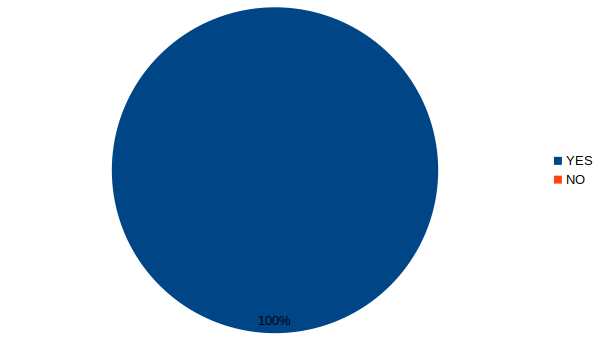
\includegraphics[width=0.5\textwidth]{seller 2.png} 
	\caption{Graphical representation of sellers who have internet access }
	\label{myLabel}		% used to reference this figure from anywhere in the document using the \ref command. 
	\end{figure} 
\newpage 
All the sellers are having good internet connectivity in Gylapozhing market resulting in 100\% of them are able to access the internet.\newline\\[0.1cm]
3)Will you be able to trust if there is online vegetable marketing system?\newline\\[0.1cm]
\begin{table}[h]       % insert the table here (where it is declared)
		\centering
		\begin{tabular}{ | l | c | r | } \hline
		\textbf{Number of Yes} & \textbf{Number of No} & \textbf{Total Number} \\ \hline			
		10 & 1 & 11 \\ \hline
		\end{tabular}
		\caption{Displaying the number of sellers who responded yes and no respectively to above question}
		\label{3.0}
	\end{table}
\begin{figure}[h]       % options: t for top of page, b for bottom, h for current position
	\centering
	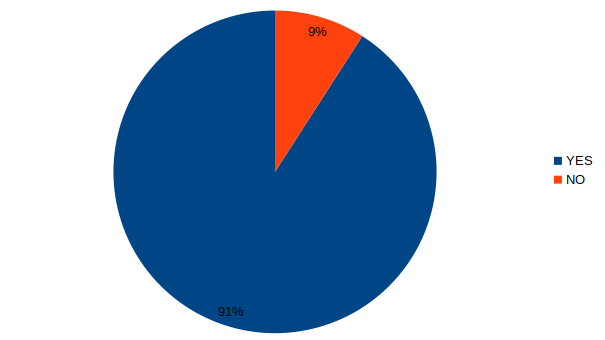
\includegraphics[width=0.5\textwidth]{seller 3.png} 
	\caption{Graphical representation seller who trust online vegetable marketing  }
	\label{myLabel}		% used to reference this figure from anywhere in the document using the \ref command. 
	\end{figure} 
\newline\\[0.1cm]Of 11 sellers, 10 of them are convinced and have trust in online vegetable marketing and one of them disagreed and does not trust online vegetable marketing resulting in 91\% yes and 9\% no.\newline\\[0.1cm]
\newpage
{\bfseries Farmers }\newline\\[0.1cm]
1)Do you have any knowledge about the online application ?\newline\\[0.1cm]
\begin{table}[h]       % insert the table here (where it is declared)
		\centering
		\begin{tabular}{ | l | c | r | } \hline
		\textbf{Number of Yes} & \textbf{Number of No} & \textbf{Total Number} \\ \hline			
		14 & 8 & 22 \\ \hline
		\end{tabular}
		\caption{Displaying the number of farmers who responded yes and no respectively to above question}
		\label{4.0}
	\end{table}
\begin{figure}[h]       % options: t for top of page, b for bottom, h for current position
	\centering
	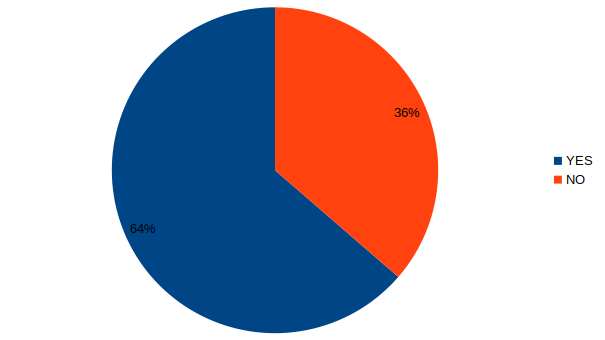
\includegraphics[width=0.5\textwidth]{farmer 1.png} 
	\caption{Graphical representation of farmers those who have knowledge about online application }
	\label{myLabel}		% used to reference this figure from anywhere in the document using the \ref command. 
	\end{figure}
\newline\\[0.1cm]Of 22 farmers 14 of them resulting 64\% are knowing online applications and 8 of them resulting in 36\% of them are not knowing online application.\newline\\[0.1cm]
2)Are you able to access internet from your place?\newline\\[0.1cm]
\begin{table}[h]       % insert the table here (where it is declared)
		\centering
		\begin{tabular}{ | l | c | r | } \hline
		\textbf{Number of Yes} & \textbf{Number of No} & \textbf{Total Number} \\ \hline			
		20 & 2 & 22 \\ \hline
		\end{tabular}
		\caption{Displaying the number of farmers who responded yes and no respectively to above question}
		\label{5.0}
	    \end{table}
\begin{figure}[h]       % options: t for top of page, b for bottom, h for current position
	\centering
	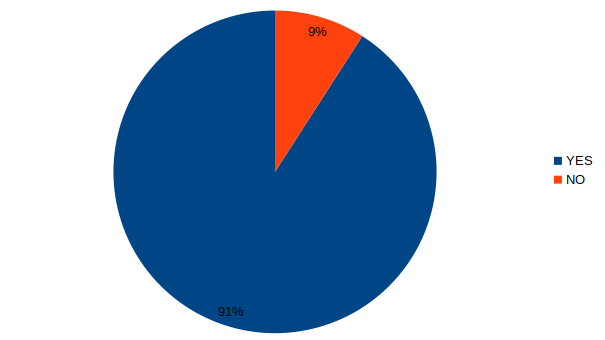
\includegraphics[width=0.5\textwidth]{farmer 2.png} 
	\caption{Graphical representation of farmers those who have internet access }
	\label{myLabel}		% used to reference this figure from anywhere in the document using the \ref command. 
	\end{figure}
	\newpage
Out of 22 farmers, 20 of them resulting in 91\% are able to access the internet, and 2 of them resulting in 9\% of them are not able to access the internet from their place.\newline\\[0.1cm]	
3)Will you be able to trust if there is online vegetable marketing system?\newline\\[0.1cm]
\begin{table}[h]       % insert the table here (where it is declared)
		\centering
		\begin{tabular}{ | l | c | r | } \hline
		\textbf{Number of Yes} & \textbf{Number of No} & \textbf{Total Number} \\ \hline			
		14 & 8 & 22 \\ \hline
		\end{tabular}
		\caption{Displaying the number of farmers who responded yes and no respectively to above question}
		\label{5.0}
	    \end{table}
\begin{figure}[h]       % options: t for top of page, b for bottom, h for current position
	\centering
	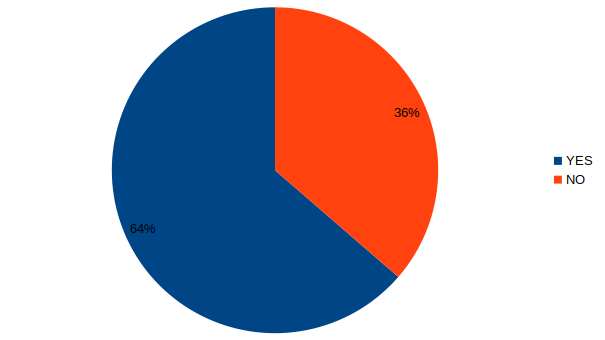
\includegraphics[width=0.5\textwidth]{farmer 3.png} 
	\caption{ Graphical representation of farmer those who trust online vegetable marketing  }
	\label{myLabel}		% used to reference this figure from anywhere in the document using the \ref command. 
	\end{figure}
\newpage
Of 22 sellers 14 of them are convinced and have trust in online vegetable marketing and 8 of them disagreed and dose not trusts online vegetable marketing resulting in 64\% “yes” and 36\% of them “no”.\newline\\[0.1cm]

{\bfseries Customers }\newline\\[0.1cm]
1)Do you have any knowledge about the online application ?\newline\\[0.1cm]
\begin{table}[h]       % insert the table here (where it is declared)
		\centering
		\begin{tabular}{ | l | c | r | } \hline
		\textbf{Number of Yes} & \textbf{Number of No} & \textbf{Total Number} \\ \hline			
		27 & 7 & 34 \\ \hline
		\end{tabular}
		\caption{Displaying the number of farmers who responded yes and no respectively to above question}
		\label{5.0}
	    \end{table}
\begin{figure}[h]       % options: t for top of page, b for bottom, h for current position
	\centering
	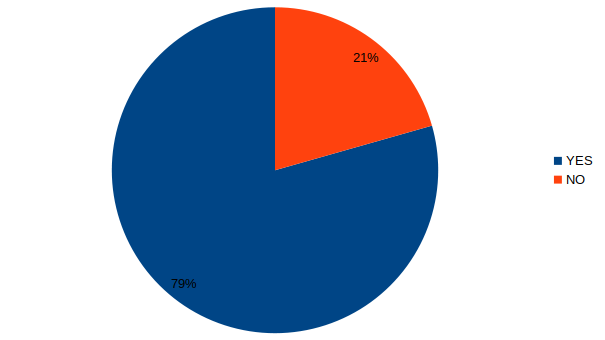
\includegraphics[width=0.5\textwidth]{customer 1.png}
	\caption{ Graphical representation of customer those who have knowledge about online application  }
	\label{myLabel}		% used to reference this figure from anywhere in the document using the \ref command. 
	\end{figure}
\newline\\[0.1cm]
Of 34 customers 27 of them resulting 79\% are knowing online applications and 7 of them resulting 21\% of them are not knowing online application.\newline\\[0.1cm]
2)Are you able to access internet from your place?\newline\\[0.1cm]
\begin{table}[h]       % insert the table here (where it is declared)
		\centering
		\begin{tabular}{ | l | c | r | } \hline
		\textbf{Number of Yes} & \textbf{Number of No} & \textbf{Total Number} \\ \hline			
		32 & 2 & 34 \\ \hline
		\end{tabular}
		\caption{Displaying the number of farmers who responded yes and no respectively to above question}
		\label{5.0}
	    \end{table}
\begin{figure}[h]       % options: t for top of page, b for bottom, h for current position
	\centering
	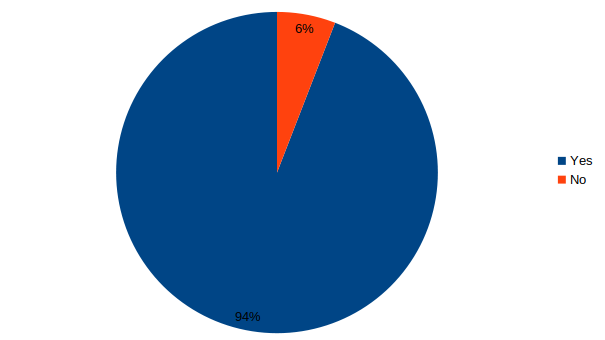
\includegraphics[width=0.5\textwidth]{customer 2.png}
	\caption{ Graphical representation of customer those who have internet access }
	\label{myLabel}		% used to reference this figure from anywhere in the document using the \ref command. 
	\end{figure}
	\newpage
Out of 34 customers, 32 of them resulting 94\% are able to access the internet, and 2 of them resulting in 6\% of them are not able to access the internet from their place.\newline\\[0.1cm]
3)Will you be able to trust if there is online vegetable marketing system?\newline\\[0.1cm]
\begin{table}[h]       % insert the table here (where it is declared)
		\centering
		\begin{tabular}{ | l | c | r | } \hline
		\textbf{Number of Yes} & \textbf{Number of No} & \textbf{Total Number} \\ \hline			
		25 & 9 & 34 \\ \hline
		\end{tabular}
		\caption{Displaying the number of farmers who responded yes and no respectively to above question}
		\label{5.0}
	    \end{table}
\begin{figure}[h]       % options: t for top of page, b for bottom, h for current position
	\centering
	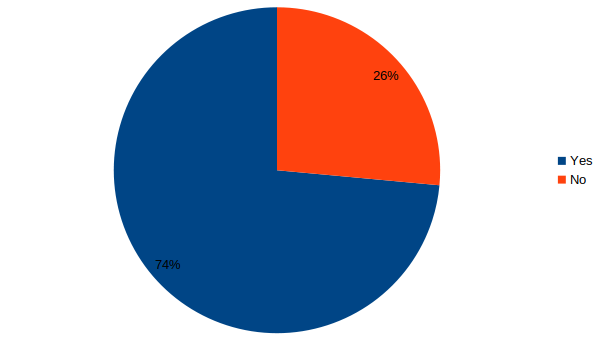
\includegraphics[width=0.5\textwidth]{customer 3.png}
	\caption{ Graphical representation of customer those who trust online vegetable marketing }
	\label{myLabel}		% used to reference this figure from anywhere in the document using the \ref command. 
	\end{figure}
\newline\\[0.1cm]Of 34 customers 25 of them are convinced and have trust in online vegetable marketing and 9 of them disagreed and dose not trust online vegetable marketing resulting in 74\% said “yes” and 26\% of them said “no”.\newline\\[0.1cm]
\newpage
\begin{figure}[h]       % options: t for top of page, b for bottom, h for current position
	\centering
	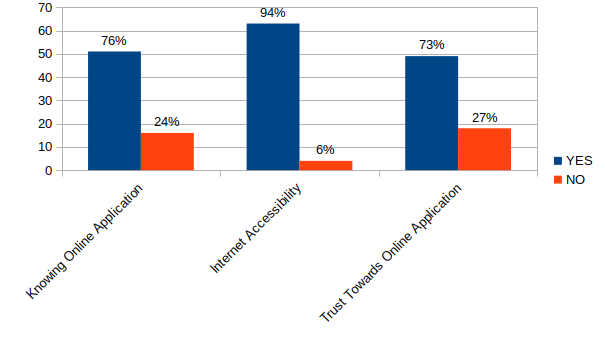
\includegraphics[width=0.7\textwidth]{finala.png}
	\caption{ Over percentage of knowledge on online application, internet accessibility, and trust towards online vegetable market }
	\label{myLabel}		% used to reference this figure from anywhere in the document using the \ref command. 
	\end{figure}
\newline6After adding the count of farmers, sellers, and customers together it counted 67, and out of 67, 76\% of them are knowing online applications and 24\% of them are not knowing the online application. Similarly, 94\% of them are able to access the internet from their residential area and only 6\% of them are not able to access the internet. Also, 73\% of them are having trust in online vegetable marketing when the team explained about online vegetable marketing  to them and 27\% of them are not having trust in online vegetable marketing.\newline\\[0.1cm]
{\bfseries Qualitative Analysis}\newline\\[0.1cm]
Besides the feasibility of online vegetable marketing in Gyalpozhing, the team has also focused on the reaction and views of farmers, sellers, and customers over the online vegetable market. Additionally, problems and challenges faced by all of them were also noted and discussed thoroughly by the team.\newline\\[0.1cm]
On conducting the interview, the team came to know that most of them were happy to meet and get connected from the current vegetable marketing system but they were also worried about spreading different illnesses which they were uninformed of. The main factor contributing to this issue was a tremendous gathering and ill-advised position where they sell and buy vegetables. More significantly they were also afraid during the pandemic of covid-19 and most of them want to avoid such gatherings but as it was only the way to earn their living they have to participate in vegetable marketing. Additionally, they have also suggested that due to gathering there is high traffic congestion and it becomes challenging for the farmer as well as the seller to handle customers during huge gatherings.\newline\\[0.1cm]
Similarly, all the farmers, customers, and sellers have given feedback on current vegetable marketing stating that marketing space was limited and they want it to be expended. Besides current vegetable marketing, they were also expecting other platforms where they can promote their product and customer can buy the product in other means. Farmers were also interested in selling their product not only on weekends but also on other days because their product gets ready before they could take it to market. Those products are getting wasted and hindering the budget they get for their living.\newline\\[0.1cm]
On interpreting the mechanism of online vegetable marketing to all the sellers, customers, and farmers, most of them were interested in it and positive feedback was given. They were also convinced that such a facility can reduce their time as they do not have to visit market for selling and buying indicating that online vegetable marketing is fast and efficient.\newline\\[0.1cm]
{\bfseries Research Question And Answers}\newline\\[0.1cm]
After retrieving the information of the all the sellers, farmers and customers, the team was able to figure out possible answers for research question as following:\newline\\[0.1cm]
1. How online vegetable market satisfy the wants and need of the customer and seller?\newline\\[0.1cm]
On explaining the mechanism of online vegetable market to all the sellers, farmers, and customers, they understood that  online marketing is fast and efficient as they will be able to reverse the  products and purchase the product  online  rather than rushing to the  market. Unlike current vegetable marketing system customers don’t have to wait in queue and customers don’t have to return with empty hand.  
Similarly sometimes the products of farmers and sellers are wasted when the products are not sold on time. Therefore to overcome such challenges farmers and sellers stated that alternate means to avoid such problems would be probably online vegetable marketing system in Gyalpozhing.\newline\\[0.1cm]
2. What are the main reasons for studying the feasibility of online vegetable marketing?\newline\\[0.1cm]
In Gyalpozhing as there is no other means to market vegetable other than current vegetable marketing system, there should be alternatives to handle if one system is not working well. So the team came with the idea of online vegetable marketing system. Importantly to implement anything, first and foremost thing is to check feasibility of the system. With the idea to implement online vegetable market in Gyalpozhing the team have done study on feasibility of online vegetable marketing to improve marketing strategies. On interviewing with all the customers, farmers, and sellers, they were supportive and gave  positive feedback on online marketing which would be fast and trust worthy, effective and time efficient.\newline\\[0.1cm]
3. Will online vegetable marketing become user friendly in Gyalpozhing?\newline\\[0.1cm]
After interviewing with  farmers, sellers, and customers of Gyalpozhing, the team could figure out that from 67 of them 76\% of them are  having good knowledge about online applications and 94\% of  them are having good internet connectivity and 73\% of them have trust to online vegetable marketing. As mentioned earlier, the major factors to check the feasibility of online vegetable marketing is based on accessibility of internet, knowledge about online applications and trust towards online vegetable market. Thus, we can conclude that online vegetable marketing will become user friendly in Gyalpozhing as more of them are  qualifying the targeted criteria i.e,  more than 70\% of them have knowledge about online application, internet connectivity and trust on online vegetable marketing.\newline\\[0.1cm]
4. Do customer have interest in online marketing?\newline\\[0.1cm]
On analyzing the data collected from sellers, customers, and farmers the team found that 73\% of them are having trust on online application and if there is trust than one will definitely have interest. Additionally they were very supportive and stated that they would be glad if such system are introduced to them because it would be alternate means for marketing. They were also interested  on online vegetable marketing because they were convinced that online vegetable marketing would be fast and efficient.\newline\\[0.1cm]
\newpage
\chapter{Conclusion and Recommendation}	
\label{chapter_conclusion}
We the team have taken three major factors namely knowledge of online applications, internet access, and trust in online vegetable marketing to check the feasibility of online vegetable marketing in Gyalpozhing. To detail the factors which help to figure out the feasibility of online vegetable marketing, firstly it is must that everybody who all are taking part in vegetable marketing should have an idea about the online application because new marketing strategies will be fully based on online application.\newline\\[0.1cm]
Similarly, internet access was also taken major factor to check the feasibility of online vegetable marketing because the internet plays an overall role in online vegetable marketing whereas without internet one cannot do online marketing. Thus the internet plays a very important role in marketing online. Finally to do online marketing one should have trust in online marketing. Without having trust over online marketing we cannot proceed with online marketing, so it becomes necessary for all the sellers, farmers and customers to have trust over online marketing.\newline\\[0.1cm]
After analyzing the data which was noted during the interview, the team came to the conclusion that online vegetable marketing is feasible in the Gyalpozhing market. It is so because  more of them were qualifying the targeted criteria i.e, more than 70\% of them were knowing the about online application, internet was accessible  from their residential area and  they are having trust on online vegetable marketing system .\newline\\[0.1cm]
Additionally, as expected we the team came to know that vegetable marketing would reduce the marketing time for all of them and it would be efficient and fast as compare to the current vegetable marketing system. And most of them were convinced to have the facility of online vegetable marketing which would avoid unnecessary ill-advised gathering. All in all, in this research all the objectives were achieved and research questions were answered.\newline\\[0.1cm]
{\bfseries Recommendation }\newline\\
After conducting research on feasibility of online vegetable marketing in Gyalpozhing, we the team would like to recommend some tips on checking the feasibility of online vegetable market. To do research on such topics, researcher should keep in mind that weather it be possible in terms of budgets, frame time, technical capabilities, financially viable and weather  it will be accepted by community. Such question helps researcher to determine whether the plan is feasible or not.Additionally, when researcher proceeds with the research it is must that  one should have good knowledge about sampling techniques and methods, and analysis methods.To be specific, if researcher wants to do determine feasibility, we recommend that it would be good to use predictive analysis as it favors in answering the questions of future outcome. Similarly for data sampling method, it would be easy and effective for the researcher to use simple random sampling.\newline\\[0.1cm]
Researchers have to be cautious while collecting data and data should be relevant to objectives and hypothesis of the research. Researchers should be aware of research method like survey, questionnaires , interviews and etc. To determine feasibility we recommend researchers to use interviews and survey because in such methods researcher can get data through live interaction. And such data are considered to be more precise and accurate resulting correct result.

%---------------------------------------------------------
%	6. References 
%---------------------------------------------------------		

% All references must appear here in APA style. You are expected to add more to the readings you used for the proposal document. Remember that credibility of your sources matters. 

\begin{thebibliography}{99}			% this environment is used for including references. Upto 99 citations are possible this way. Instead of key1, key2..., you can give your own key name. 
	
	\bibitem{key1}Greene, W. H. (2000). E conometric Analysis. Prentice-Hall, USA. 
	
	\bibitem{key2} Gil, J. M., Gracia A., Sanchez, M. (2000). Market segmentation and willingness to pay for organic
    products in Spain. International Food and Agribusiness Management Review, 3(2), 207-226.
    \bibitem{key3}Carmer(2012).journal hunger & Environment Nutrition. retreived from https://tandfonline.com/
    \bibitem{key4}Sonam(2018, June 2).Graduates start online vegetable shopping. retreived from https://kuenselonline.com/grad-start-online-vegetable-shopping/
    
	

\end{thebibliography}



\newpage



%---------------------------------------------------------
%	Apprendix
%---------------------------------------------------------		
\chapter*{Appendix}
Captured video of interview, visit link to view the video:
\newline\\[0.1cm]
\href{https://www.dropbox.com/s/zhjewbta4r5x05z/DSC_0437.MOV?dl=0}{Click this link to see interview with --Customer}.
\newline\\[0.1cm]
\href{https://www.dropbox.com/s/l2rd9ojg9kzjbfl/DSC_0457.MOV?dl=0}{Click this link to see interview with --Seller}.




\end{normalsize}
	
	
		
	
\end{document}
